\section{SVM}
\subsection{Classification}
\begin{frame}{Classification problem}
	\begin{itemize}\setlength\itemsep{1em}
		\item[Goal:] To produce a classifier able to decide whether an object belongs to one or more classes.
		\item[Idea:] Supervised Learning: Given a dataset of already classified examples, the classifier \textit{learns} a function that solves classification problem.
	\end{itemize}
\end{frame}

\begin{frame}{Notation}
	Dataset is set of classified examples:
	$$D = \{(X_i, Y_i) | \ i \in [1, n]\}$$
	$$X_i \in \R^f$$
	$$Y_i \in \{-1, +1\}$$
	\begin{itemize}\setlength\itemsep{1em}
		\item A vector $x \in \mathbb{R}^f$ represents an object using $f$ \textit{relevant} features.
		\item A number $y \in \{-1 , +1\}$ indicates wether the example belong to target class.
	\end{itemize}
	
	While learning the target function, the dataset is divided in \textit{training set} and \textit{test set}.
\end{frame}

\subsection{SVM}
\begin{frame}{SVM}
	\begin{itemize}\setlength\itemsep{1em}
		\item The idea is to compute the \textit{maximum-margin hyperplane} $w^Tx + b$ which best separates positive examples from negative examples.
	\end{itemize}
	\begin{columns}
		\begin{column}{0.5\textwidth}\centering
			Optimization problem is:
			$$arg min_w \frac{1}{2} ||w||^2$$
			$$Y_i (w^T X_i + b) \geq 1 \ \forall i \in [1, n]$$
		\end{column}
		\begin{column}{0.5\textwidth}\centering
			\begin{figure}[htbp]
				\centering
				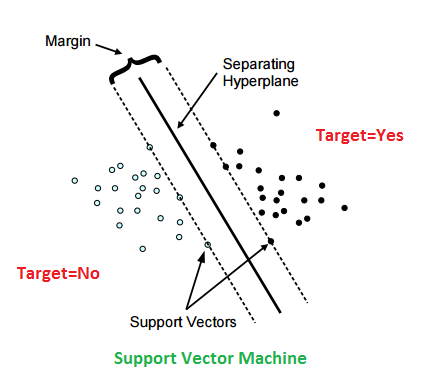
\includegraphics[scale = 0.40]{./images/optimal-hyperplane2.png}
				\caption{\textit{Solution of maximum-margin hyperplane}}
			\end{figure}
		\end{column}
	\end{columns}
	
	
	
\end{frame}

\begin{frame}{SVM with slacks}
	\begin{itemize}\setlength\itemsep{1em}
		\item The examples may not be linearly serparable and so the problem would not have any solutions because constraints are not satisfied. Then we introduce slack variables $\xi$
	\end{itemize}
	\begin{columns}
		\begin{column}{0.5\textwidth}\centering
			Optimization problem becomes:
			$$arg min_{w, \xi} \frac{1}{2} ||w||^2 + C \sum_{i = 1}^{n}\xi_i$$
			$$y_i (w^T x_i + b) \geq 1 - \xi_i \ \forall i \in [1, n]$$
			$$\xi_i \geq 0 \ \forall i \in [1, n]$$
		\end{column}
		\begin{column}{0.5\textwidth}\centering
			\begin{figure}[htbp]
				\centering
				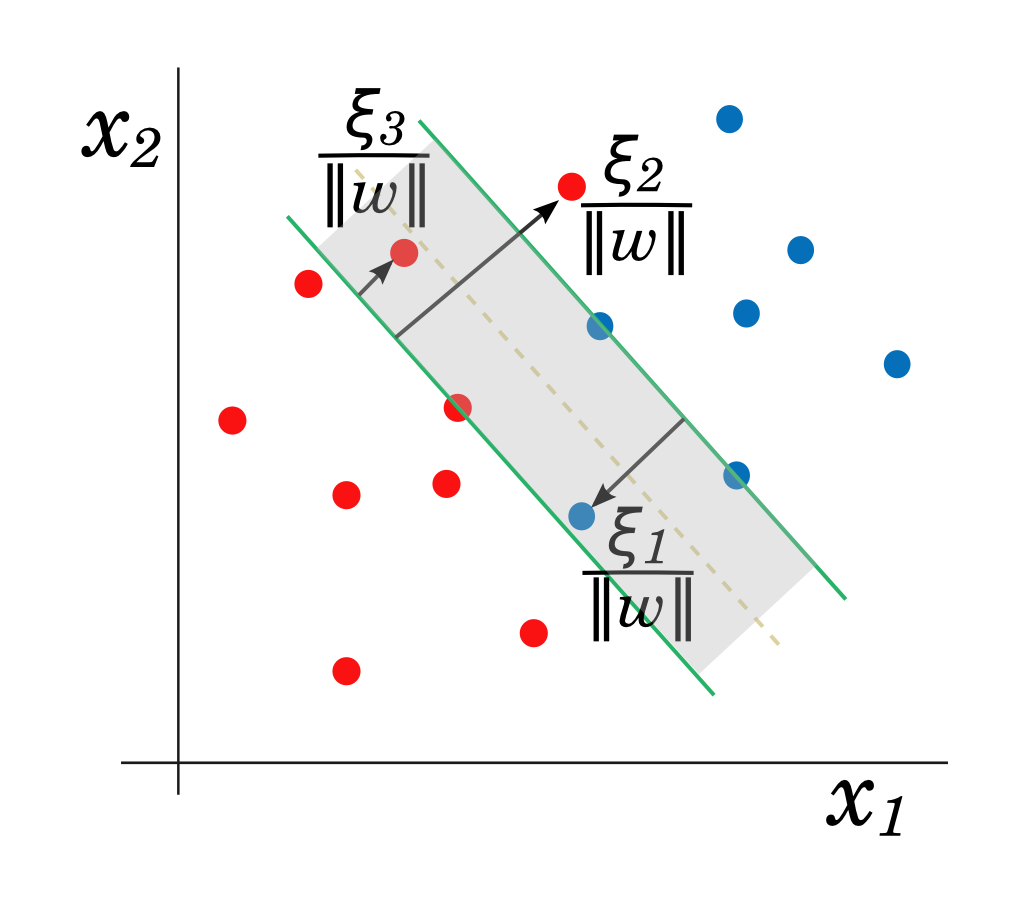
\includegraphics[scale = 0.15]{./images/slack2.png}
				\caption{\textit{Solution with slacks}}
			\end{figure}
		\end{column}
	\end{columns}
	
\end{frame}